% Created 2024-04-09 mar 07:20
% Intended LaTeX compiler: pdflatex
\documentclass[aspectratio=169, usenames,svgnames,dvipsnames]{beamer}
\usepackage[utf8]{inputenc}
\usepackage[T1]{fontenc}
\usepackage{graphicx}
\usepackage{longtable}
\usepackage{wrapfig}
\usepackage{rotating}
\usepackage[normalem]{ulem}
\usepackage{amsmath}
\usepackage{amssymb}
\usepackage{capt-of}
\usepackage{hyperref}
\usepackage{color}
\usepackage{listings}
\usepackage{mathpazo}
\usepackage{gensymb}
\usepackage{amsmath}
\usepackage{diffcoeff}
\usepackage{steinmetz}
\usepackage{mathtools}
\usepackage{fancyvrb}
\DefineVerbatimEnvironment{verbatim}{Verbatim}{fontsize=\tiny, formatcom = {\color{black!70}}}
\bibliographystyle{plain}
\usepackage{siunitx}
\sisetup{per-mode=symbol}
\sisetup{output-decimal-marker={,}}
\DeclareSIUnit{\watthour}{Wh}
\DeclareSIUnit{\wattpeak}{Wp}
\DeclareSIUnit{\watthour}{Wh}
\DeclareSIUnit{\amperehour}{Ah}
\usepackage{steinmetz}
\hypersetup{colorlinks=true, linkcolor=Blue, urlcolor=Blue}
\usepackage[symbol, perpage]{footmisc}
\parskip=5pt
\usepackage{tikz}
\usetheme{Boadilla}
\usecolortheme{rose}
\usefonttheme{serif}
\author{\href{https://oscarperpinan.github.io}{Oscar Perpiñán Lamigueiro}}
\date{}
\title{Variabilidad de la Potencia de una Central Fotovoltaica}
\subtitle{Energía Solar Fotovoltaica}
\institute[UPM]{Universidad Politécnica de Madrid}
\setbeamercolor{alerted text}{fg=blue!50!black} \setbeamerfont{alerted text}{series=\bfseries}
\AtBeginSubsection[]{\begin{frame}[plain]\tableofcontents[currentsubsection,sectionstyle=show/hide,subsectionstyle=show/shaded/hide]\end{frame}}
\AtBeginSection[]{\begin{frame}[plain]\tableofcontents[currentsection,hideallsubsections]\end{frame}}
\beamertemplatenavigationsymbolsempty
\setbeamertemplate{footline}[frame number]
\setbeamertemplate{itemize items}[triangle]
\setbeamertemplate{enumerate items}[circle]
\setbeamertemplate{section in toc}[circle]
\setbeamertemplate{subsection in toc}[circle]
\hypersetup{
 pdfauthor={\href{https://oscarperpinan.github.io}{Oscar Perpiñán Lamigueiro}},
 pdftitle={Variabilidad de la Potencia de una Central Fotovoltaica},
 pdfkeywords={},
 pdfsubject={},
 pdfcreator={Emacs 29.1 (Org mode 9.6.11)}, 
 pdflang={Spanish}}
\begin{document}

\maketitle

\section{Introducción}
\label{sec:org7795e04}

\subsection{Los Sistemas Fotovoltaicos y la Red Eléctrica}
\label{sec:orga0da1a7}

\begin{frame}[label={sec:org9dd7afd}]{Alteración de las condiciones de funcionamiento de la red}
Los sistemas fotovoltaicos conectados a red alteran las condiciones de
funcionamiento habitual de la red.

\begin{itemize}
\item Bidireccionalidad del flujo de potencia
\item Rampas de potencia
\item Servicios de apoyo
\end{itemize}

\begin{center}
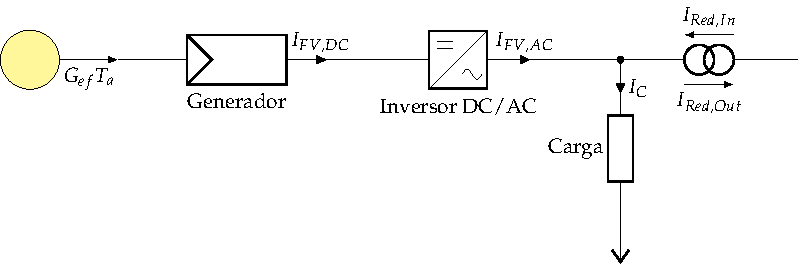
\includegraphics[width=\textwidth]{../figs/SFCR_bidireccional.pdf}
\end{center}
\end{frame}

\begin{frame}[label={sec:org95d56d0}]{Bidireccionalidad del flujo de potencia}
Posibilitan la \alert{bidireccionalidad del flujo de potencia}, con los
consiguientes \alert{cambios en la tensión de los nodos}, y \alert{en la corriente}
conducida por las líneas y transformadores\footnote{\url{https://dx.doi.org/10.3390/solar2010003}}.

\begin{center}
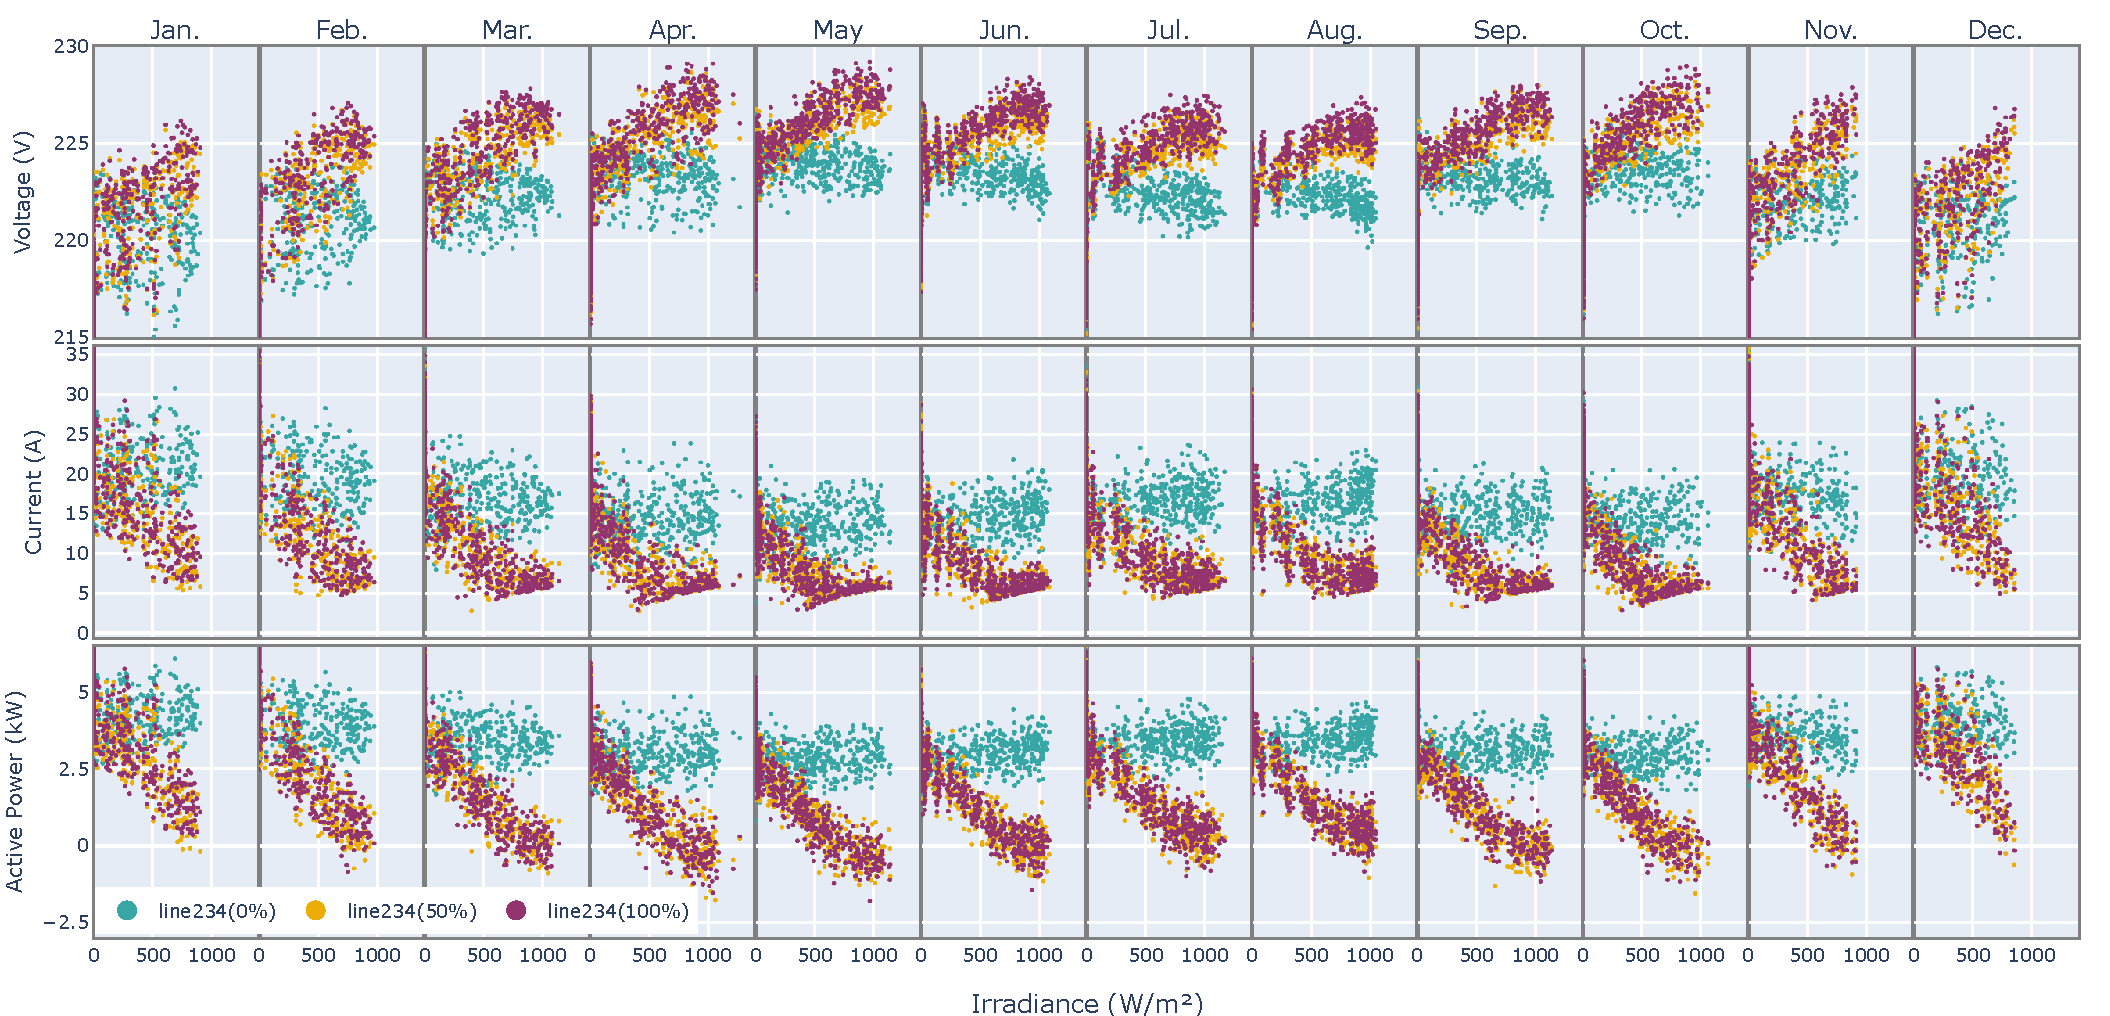
\includegraphics[height=0.65\textheight]{../figs/S_VIP_Irr_line234.pdf}
\end{center}
\end{frame}

\begin{frame}[label={sec:orgbbca917}]{Rampas de potencia}
Las \alert{rampas de potencia} debidas a las \alert{fluctuaciones de radiación solar}
pueden entorpecer el adecuado funcionamiento de los equipos
conectados a la red y los elementos de protección existentes.

\begin{center}
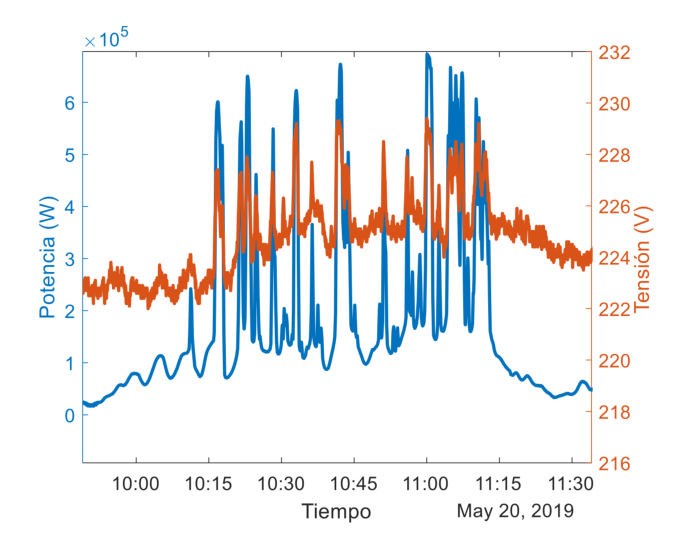
\includegraphics[height=0.75\textheight]{../figs/VariacionTension_RampasPotencia.pdf}
\end{center}
\end{frame}


\begin{frame}[label={sec:org2bc93dd}]{Servicios de apoyo a la red}
Los SFCR pueden proporcionar \alert{servicios de apoyo} a la red gracias a las
funcionalidades que incorporan los inversores de conexión a red,
capaces de \alert{controlar la potencia activa inyectada} en el punto de
conexión, \alert{y la potencia reactiva} en funcionamiento normal o para
enfrentarse a \alert{huecos de tensión}.

\begin{center}
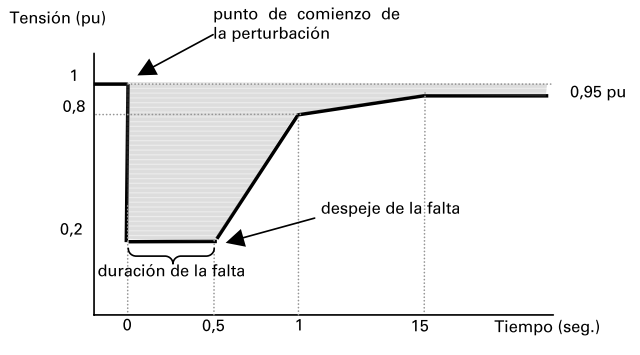
\includegraphics[height=0.7\textheight]{../figs/hueco-tension.png}
\end{center}
\end{frame}

\subsection{Variabilidad de la Radiación}
\label{sec:org2f77527}

\begin{frame}[label={sec:org9ec9f37}]{La variabilidad de la irradiancia solar}
La irradiancia solar es un \alert{proceso con inercia} que, en general, no
presenta alta probabilidad para mostrar cambios abruptos.

La \alert{probabilidad y el nivel de las fluctuaciones dependen}:
\begin{itemize}
\item de la \alert{resolución temporal},
\item del \alert{estado de la atmósfera}.
\end{itemize}
\end{frame}

\begin{frame}[label={sec:org19b19d9}]{Dependencia de la resolución temporal}
La probabilidad de ocurrencia de fluctuaciones elevadas es
sustancialmente menor al observar con resoluciones temporales
altas.

\begin{center}
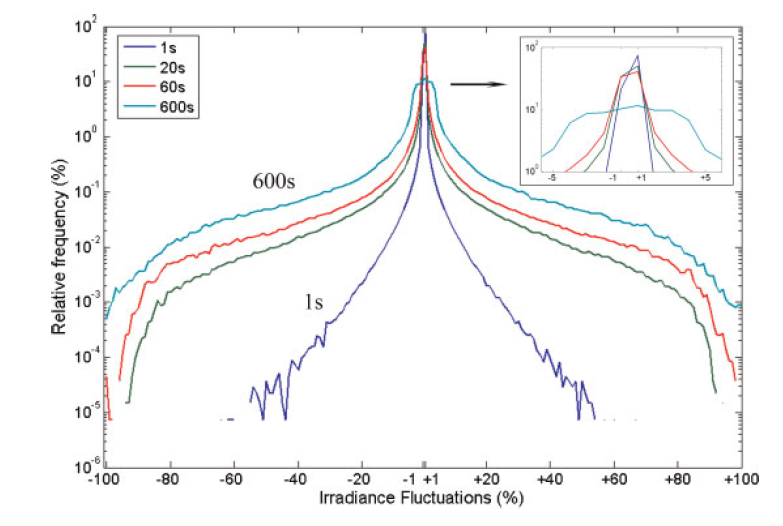
\includegraphics[height=0.75\textheight]{../figs/FluctuacionIrradiancia_Marcosetal2011.png}
\end{center}
\end{frame}

\begin{frame}[label={sec:org82c7296}]{Dependencia de la atmósfera}
El nivel de fluctuación depende del comportamiento de la atmósfera
(mayor en días parcialmente cubiertos).

\begin{center}
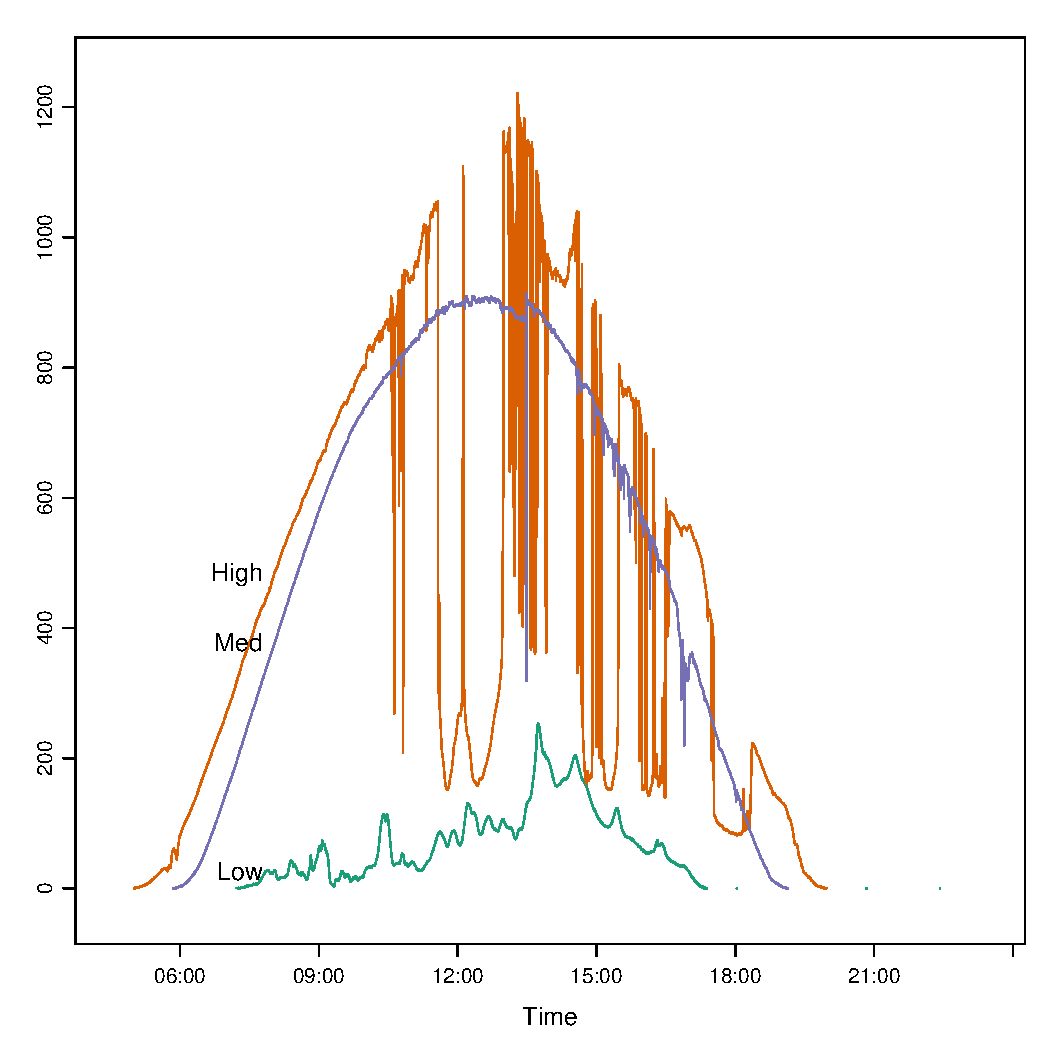
\includegraphics[height=0.8\textheight]{../figs/radLowMedHigh.pdf}
\end{center}
\end{frame}


\section{Incertidumbre y Predicción}
\label{sec:org3117434}

\subsection{Generación y Demanda}
\label{sec:orgdc72f18}
\begin{frame}[label={sec:orgd0ffefd}]{Generación y Demanda}
La \alert{casación entre generación y demanda} que se consigue en las redes
eléctricas se basa en la \alert{programación} de las diferentes unidades de
\alert{generación} disponibles para suministrar la \alert{demanda prevista} y para
constituir \alert{reservas} que hagan frente a las posibles \alert{variaciones} en la
demanda.

\begin{center}
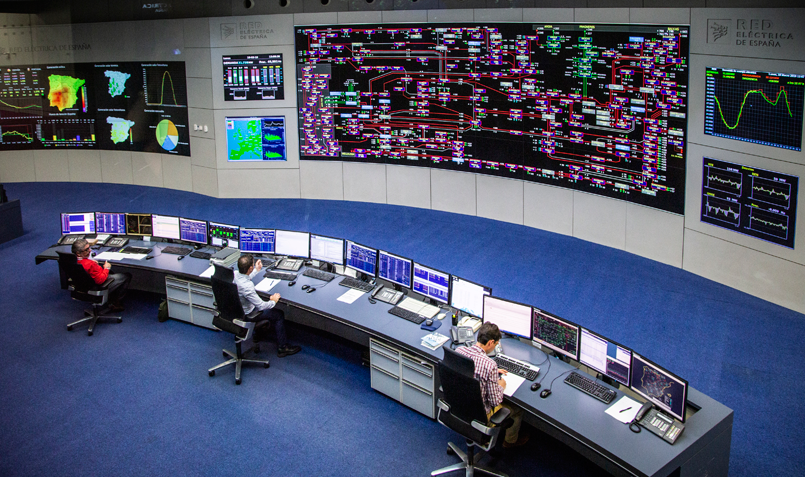
\includegraphics[height=0.65\textheight]{../figs/CentroOperacionesREE.png}
\end{center}
\end{frame}


\begin{frame}[label={sec:orgf081406}]{Programación de la generación}
Esta programación se produce en \alert{escalas y horizontes temporales diversos} y se \alert{actualiza de forma sistemática} de acuerdo con las variaciones previstas en la predicción de la demanda.

\begin{center}
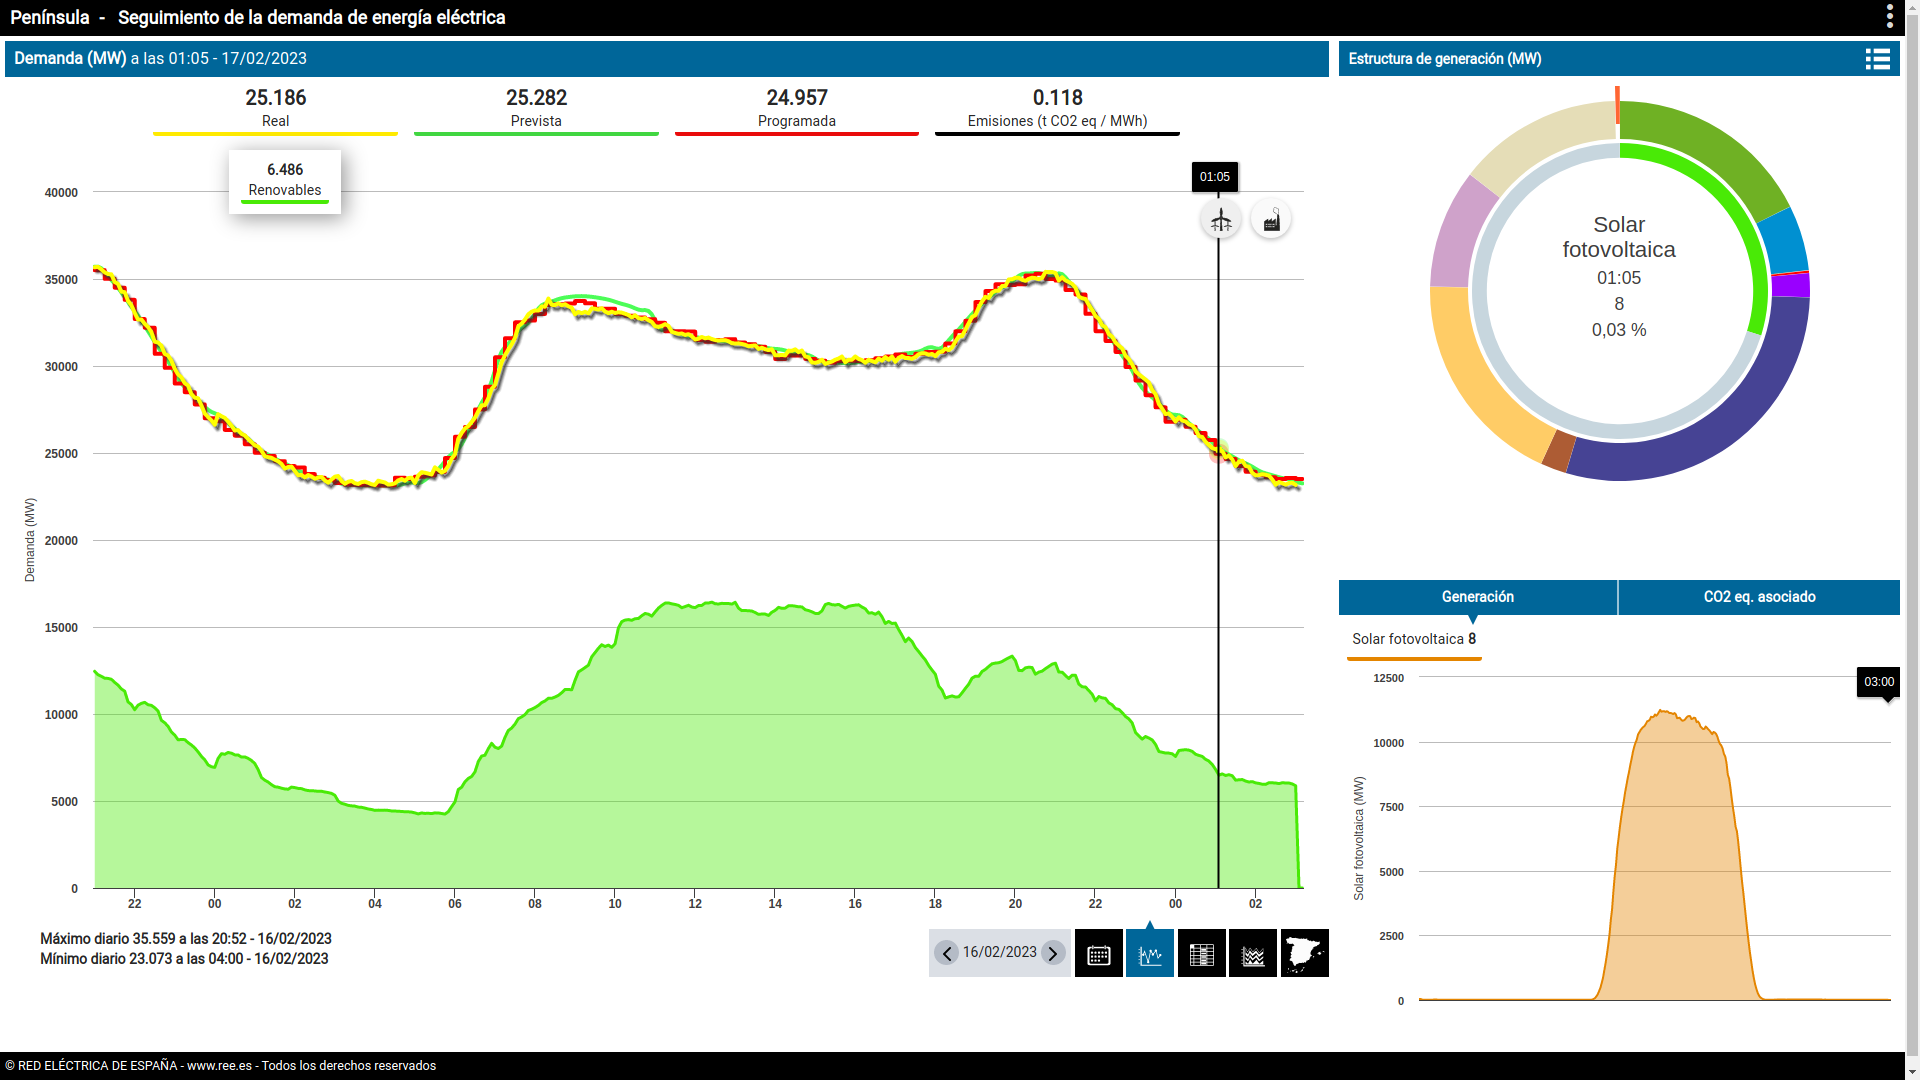
\includegraphics[height=0.6\textheight]{../figs/CurvaDemandaREE.png}
\end{center}

\begin{center}
\url{https://demanda.ree.es/visiona/peninsula/demandaqh/total/}
\end{center}
\end{frame}


\begin{frame}[label={sec:orge597626}]{Participación masiva de la fotovoltaica}
La \alert{inclusión masiva} de sistemas fotovoltaicos en la red \alert{modifica el
equilibrio} existente y puede implicar el uso de las reservas de
generación previstas originalmente para asumir las variaciones de la
demanda.

\begin{center}
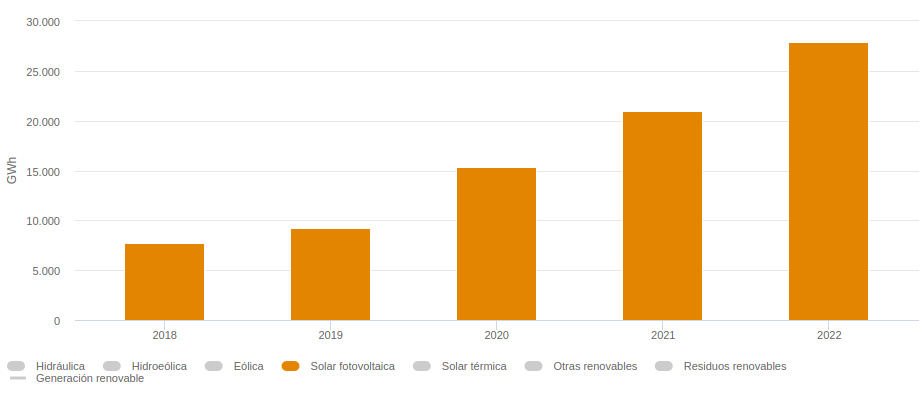
\includegraphics[height=0.6\textheight]{../figs/EvolucionGeneracionFV_REE.png}
\end{center}
\end{frame}

\subsection{Predicción de la potencia FV}
\label{sec:orgcfa97c0}
\begin{frame}[label={sec:org2f084df}]{Predicción de la Potencia}
En este contexto, el reto no es tanto la variabilidad como la
\alert{predicción}:

\begin{itemize}
\item La realización de \alert{predicciones en horizontes horarios o diarios} de
la potencia generada por un sistema fotovoltaico o por un grupo de
sistemas es \alert{crucial para facilitar la integración} de sistemas
fotovoltaicos en redes eléctricas.

\item La predicción de radiación solar y potencia de sistemas
fotovoltaicos es un \alert{área de investigación de plena actualidad}.
\end{itemize}
\end{frame}

\begin{frame}[label={sec:orgaf95315}]{Ejemplo: proyecto europeo PVCROPS}
\begin{itemize}
\item Herramienta de \alert{aprendizaje automático} o \emph{machine learning}
entrenada con \alert{series históricas} de \alert{predicciones NWP} y \alert{medidas de
potencia eléctrica} (30 días en la serie temporal de
entrenamiento)\footnote{\url{https://dx.doi.org/10.1016/j.solener.2015.03.006}}.
\item \alert{Predicción de potencia AC} con resolución \alert{horaria} y un horizonte
temporal de \alert{1 día}.
\end{itemize}


\begin{center}
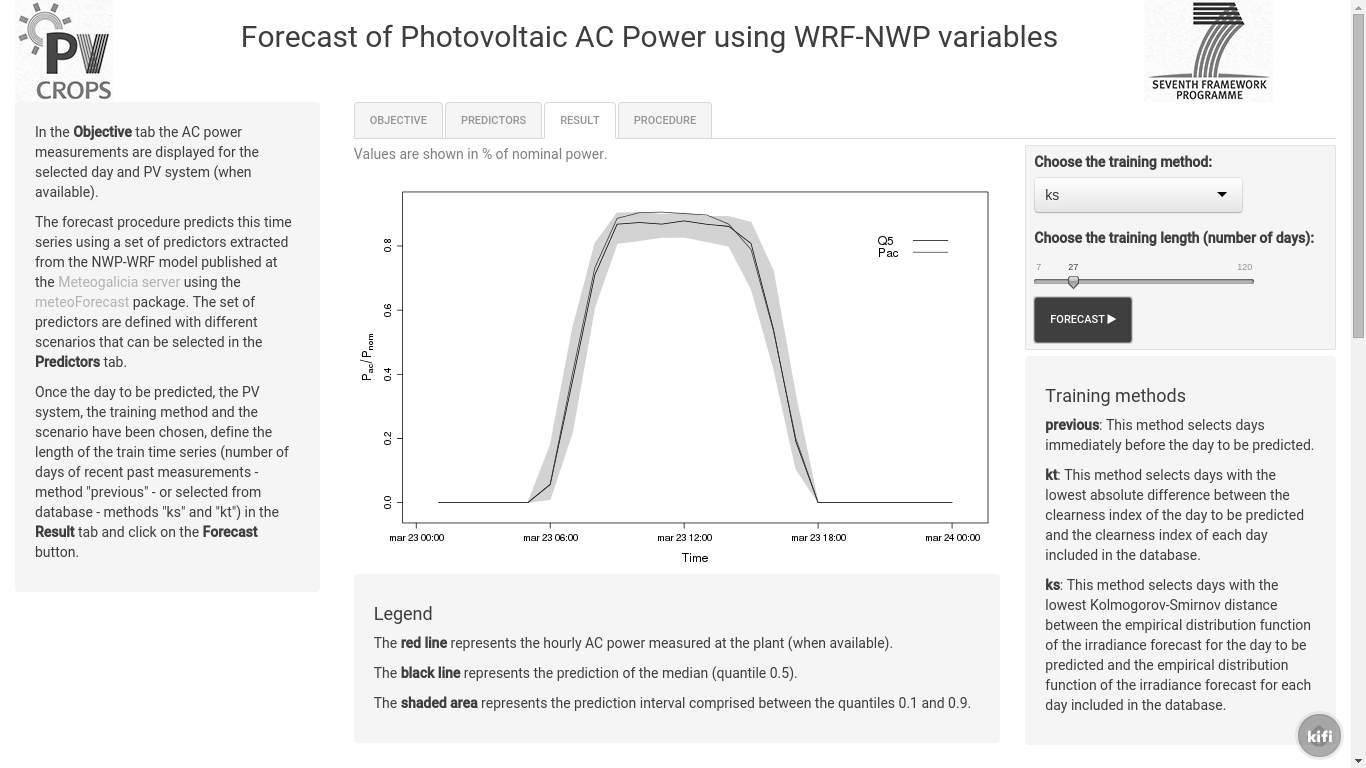
\includegraphics[height=0.6\textheight]{../figs/ForecastShiny.png}
\end{center}
\end{frame}

\begin{frame}[label={sec:orgb3e4eab}]{Ejemplo: proyecto europeo PVCROPS}
Se emplean como entradas las predicciones de \alert{variables
meteorológicas} generadas por modelos de predicción meteorológica
numérica e \alert{índices de variación espacial y temporal} estimados con
las variables meteorológicas.

\begin{center}
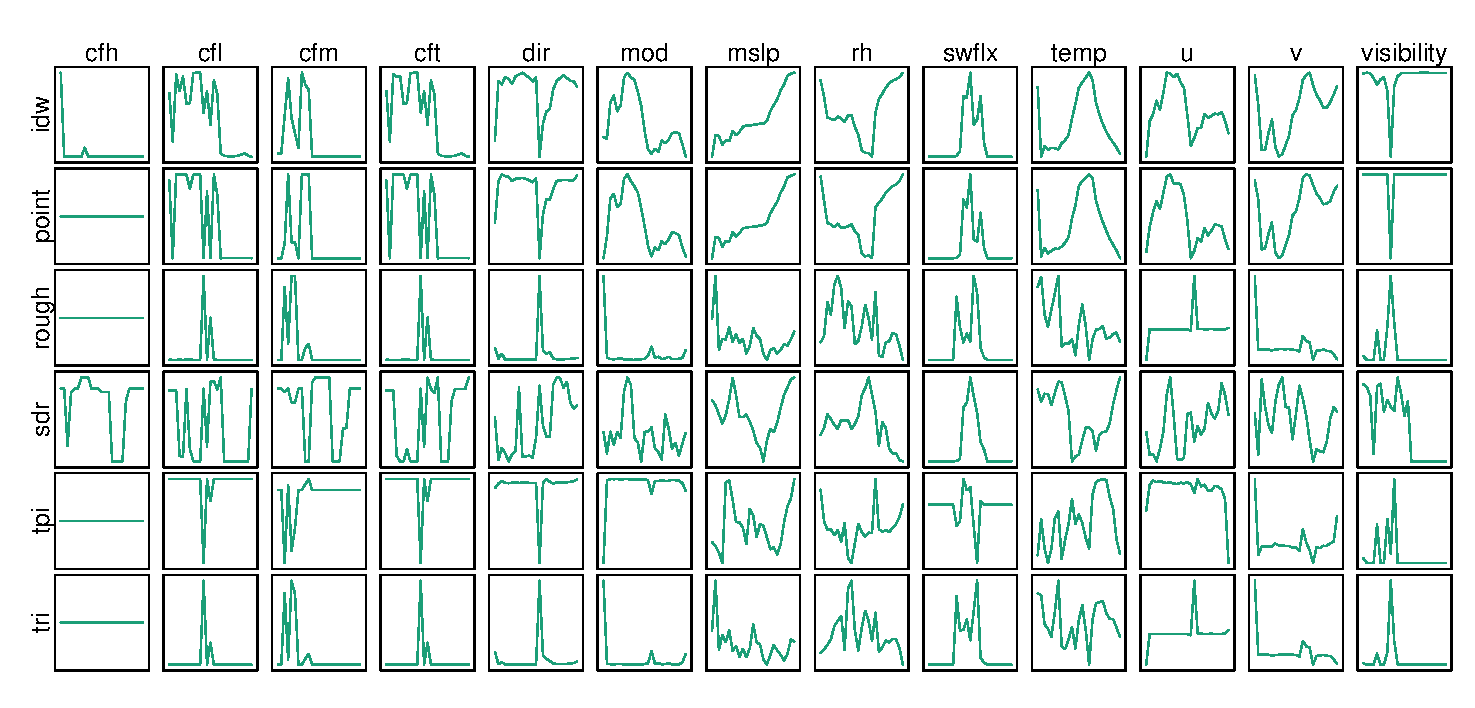
\includegraphics[height=0.7\textheight]{../figs/varsComplete.pdf}
\end{center}
\end{frame}


\begin{frame}[label={sec:org3c59c43}]{Ejemplo: proyecto europeo PVCROPS}
Genera \alert{predicciones probabilísticas}, entregando tanto la mediana de la
predicción como un intervalo de confianza, que permite cuantificar la
fiabilidad de la predicción, y que puede servir como medida indirecta
de la variabilidad futura.

\begin{center}
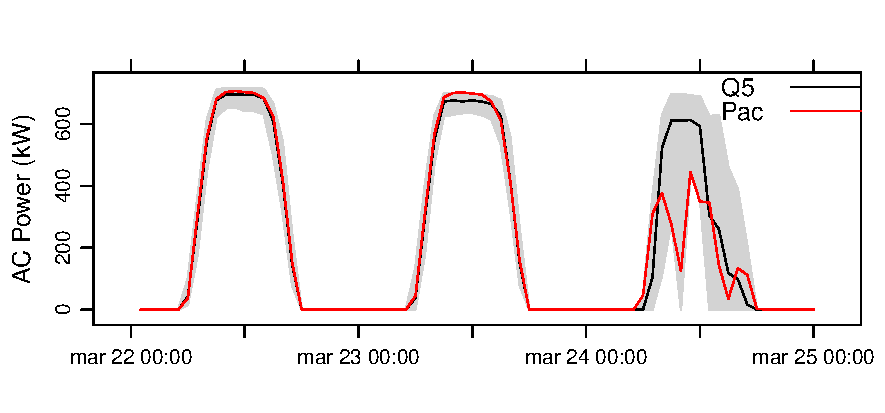
\includegraphics[width=0.6\textwidth]{../figs/powerResult.pdf}
\end{center}

\begin{center}
\url{http://vps156.cesvima.upm.es:3838/predictPac/}
\end{center}
\end{frame}


\begin{frame}[label={sec:org9ac8d3d}]{Predicciones agregadas}
Las predicciones obtenidas mejoran cuando las predicciones se aplican
a un conjunto de sistemas.\footnote{\url{https://dx.doi.org/10.1002/pip.1033}}

\begin{center}
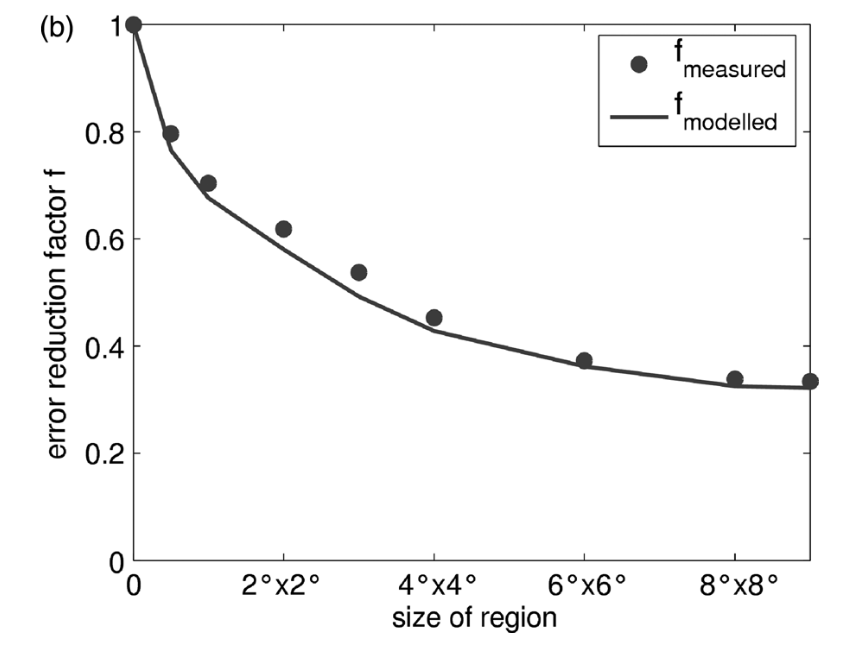
\includegraphics[height=0.7\textheight]{../figs/ForecastEnsembleErrorReduction.png}
\end{center}
\end{frame}

\section{Variabilidad de la Potencia}
\label{sec:org1a33410}

\begin{frame}[label={sec:org5ecbc90}]{Variabilidad de la potencia}
La variabilidad presente en la irradiancia solar se \alert{atenúa} en la potencia AC:
\begin{itemize}
\item por la \alert{dispersión} espacial \alert{entre diferentes centrales}.
\item por la \alert{dispersión} espacial \alert{dentro de una central}.
\end{itemize}
\end{frame}
\subsection{Dispersión espacial entre centrales}
\label{sec:org37ac106}
\begin{frame}[label={sec:org6beb027}]{Dispersión espacial entre centrales}
En términos generales, la \alert{dispersión espacial de sistemas
fotovoltaicos diferentes} conectados a la misma red \alert{atenúa} la
variabilidad conjunta\footnote{\url{https://dx.doi.org/10.1002/pip.1127}}.

\begin{center}
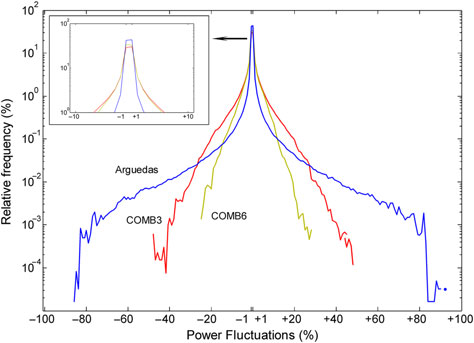
\includegraphics[height=0.7\textheight]{../figs/Variabilidad_DispersionGeografica_Plantas.png}
\end{center}
\end{frame}

\begin{frame}[label={sec:orgd98c4a9}]{Dependencia de meteorología y distancia}
El \alert{nivel de atenuación depende} principalmente:
\begin{itemize}
\item de las \alert{características meteorológicas} de la zona y época,
\item y de la \alert{distancia} entre los sistemas\footnote{Para \alert{distancias mayores de \(\SI{5}{\kilo\meter}\)} las
fluctuaciones de irradiancia con resolución temporal de 1 minuto
están esencialmente \alert{incorreladas}.}.
\end{itemize}
\end{frame}

\subsection{Dispersión espacial dentro de una central}
\label{sec:org792acf6}

\begin{frame}[label={sec:org3338da8}]{La central atenúa la potencia}
En términos generales, la \alert{dispersión espacial} de generadores
fotovoltaicos pertenecientes a \alert{una misma central} \alert{atenúa} la
variabilidad conjunta\footnote{\url{https://dx.doi.org/10.1002/pip.1016}}.

\begin{center}
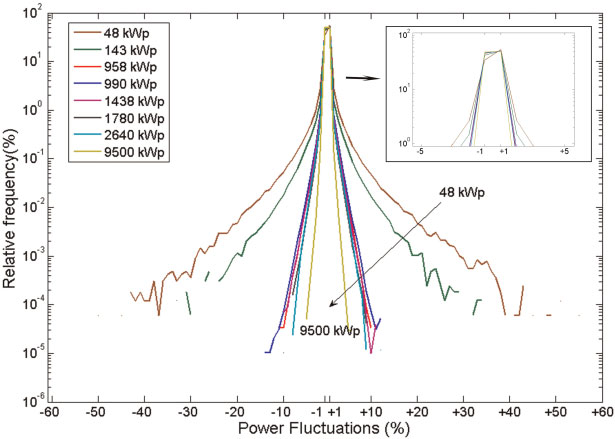
\includegraphics[height=0.7\textheight]{../figs/Variabilidad_DispersionGeografica_Planta.png}
\end{center}
\end{frame}

\begin{frame}[label={sec:orgb821313}]{Dependencia de la resolución temporal, distancia y tipo de día}
La correlación entre la potencia de cada inversor \alert{depende} de la \alert{resolución temporal}, la \alert{distancia} entre los inversores, y el \alert{nivel de fluctuación del día} en cuestión\footnote{\url{https://dx.doi.org/10.1016/j.solener.2012.12.004}}.

\begin{center}
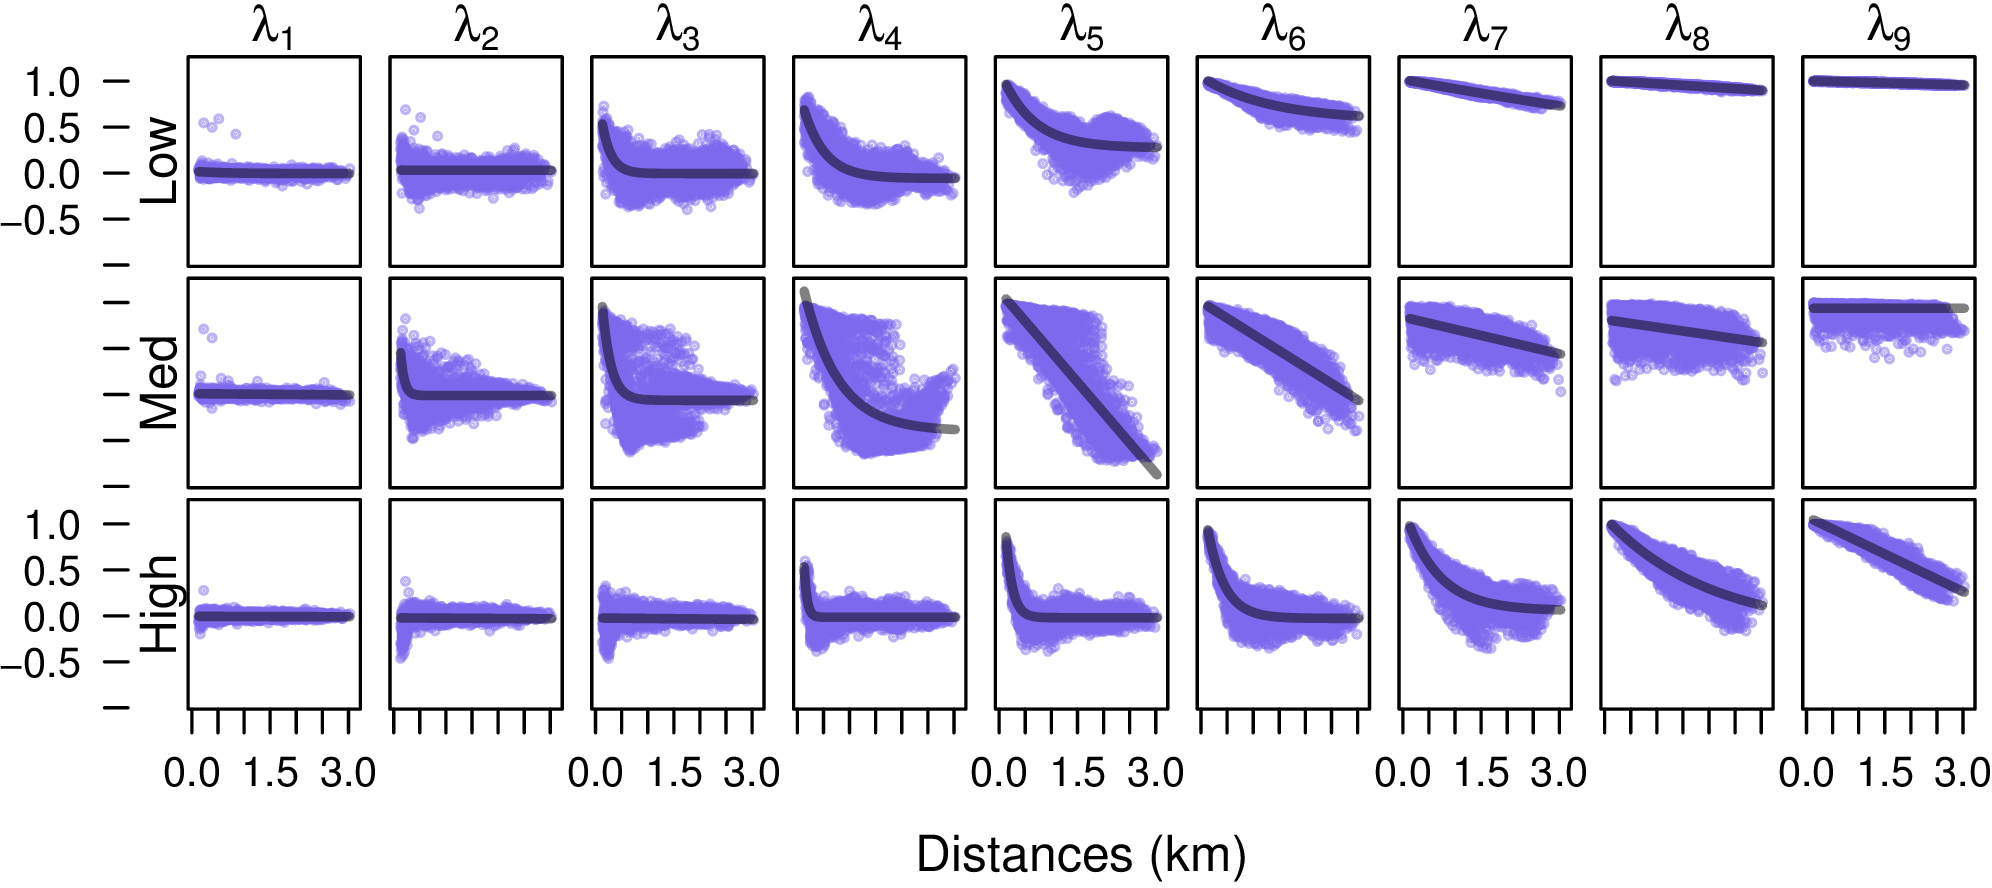
\includegraphics[height=0.6\textheight]{../figs/corDistMatrix_nls.png}
\end{center}
\end{frame}

\begin{frame}[label={sec:orga8b332e}]{Escalas temporales bajas}
Escalas temporales bajas (\(\tau <\qty{1}{\min}\)): correlaciones bajas.

\begin{center}
  \begin{tikzpicture}
    \node[anchor=south west,inner sep=0] at (0,0) {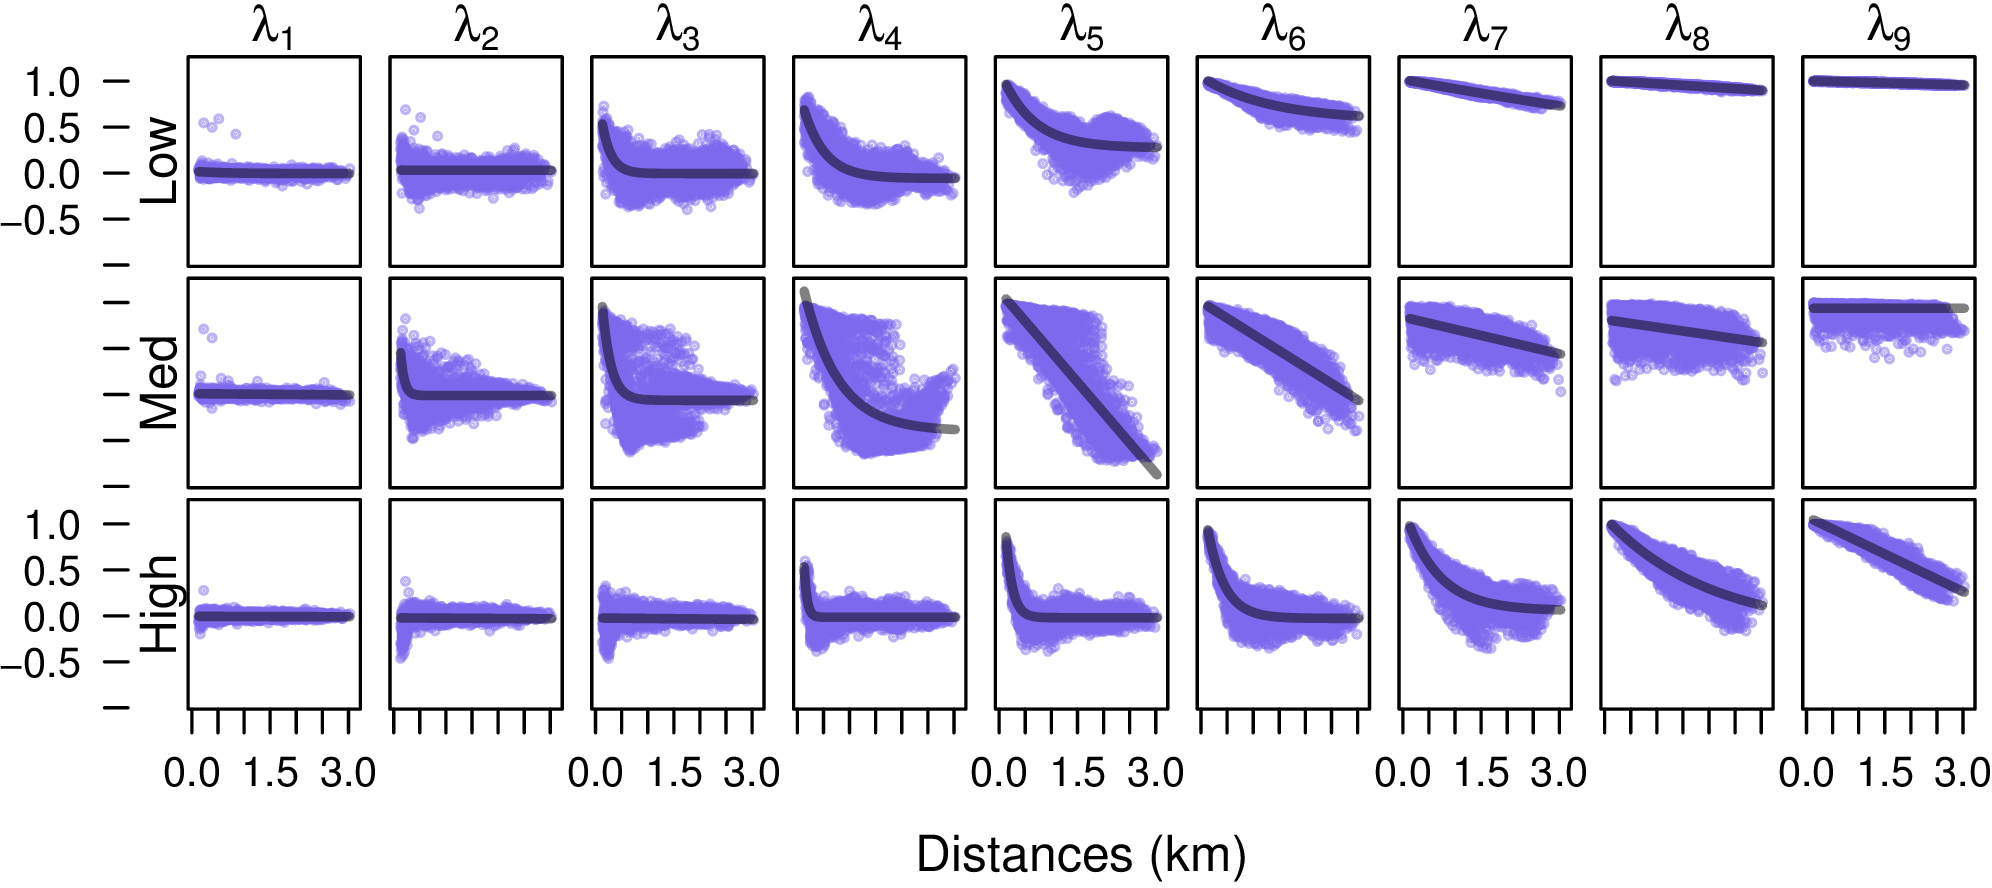
\includegraphics[height=0.5\textheight]{../figs/corDistMatrix_nls.png}};
      \draw[red,ultra thick,rounded corners] (0,0) rectangle (3, 0.55\textheight);
    \end{tikzpicture}
  \end{center}
\end{frame}

\begin{frame}[label={sec:org8409e79}]{Escalas temporales intermedias}
Escalas temporales intermedias: la correlación depende fuertemente del nivel de fluctuación diario.

\begin{center}
  \begin{tikzpicture}
    \node[anchor=south west,inner sep=0] at (0,0) {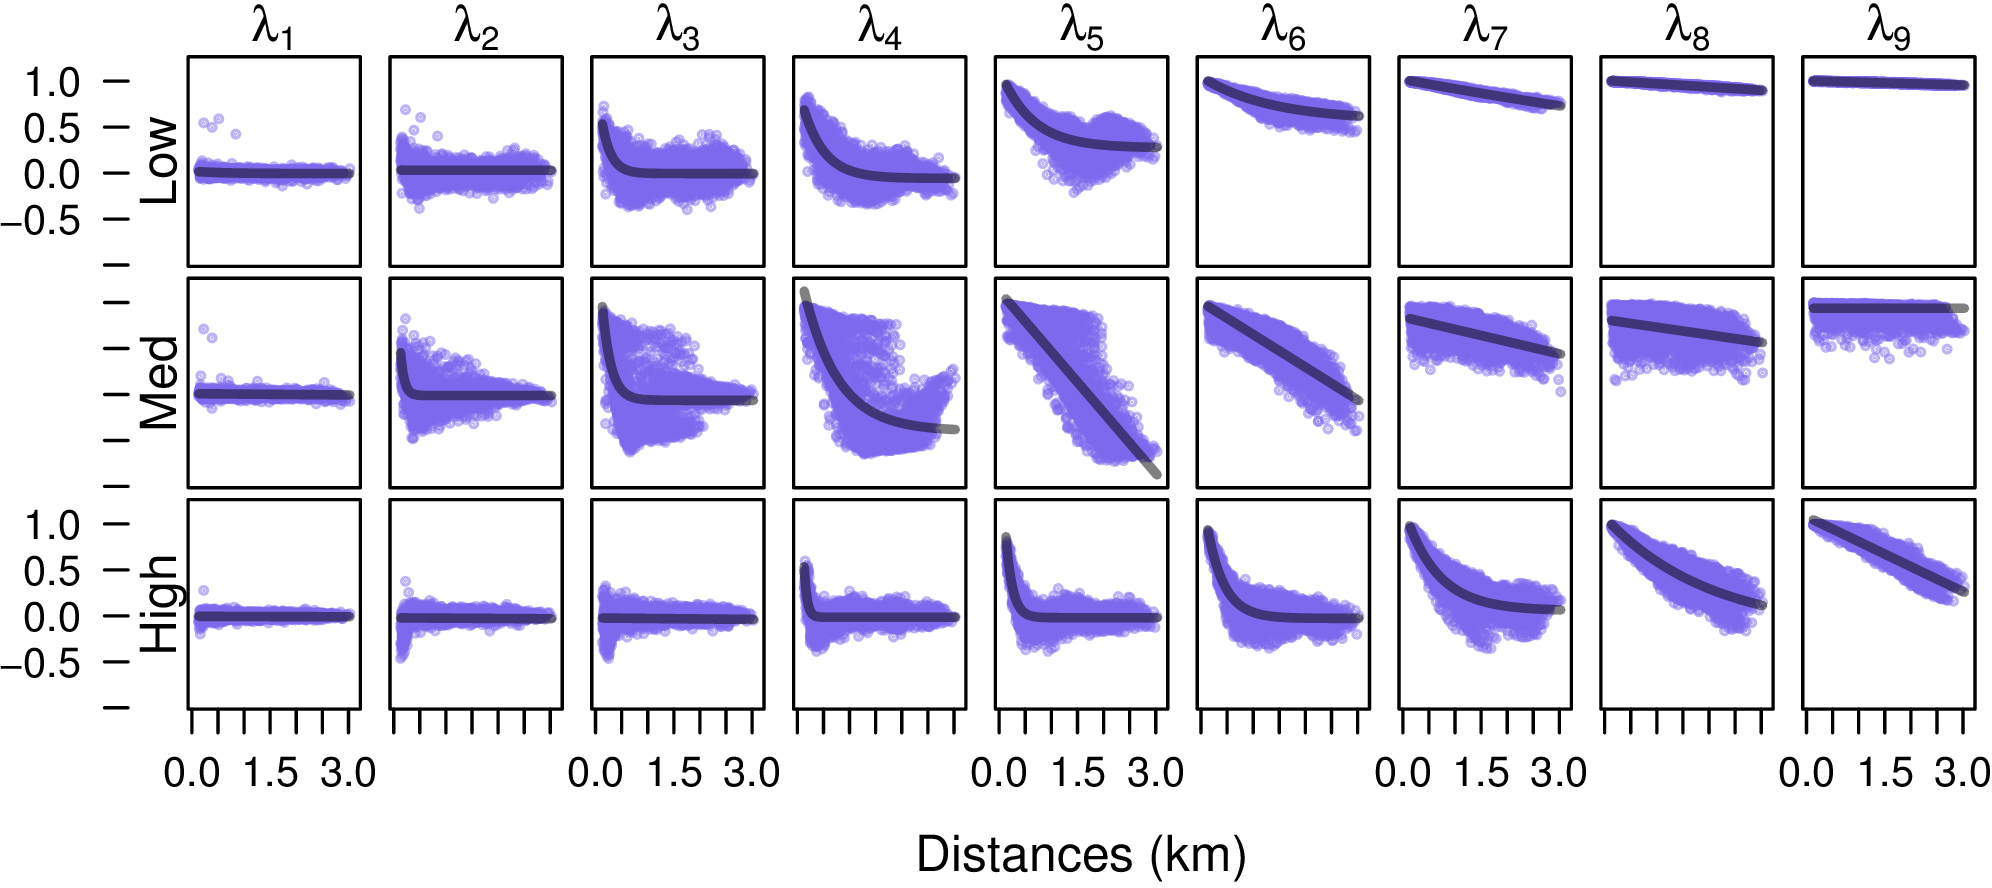
\includegraphics[height=0.5\textheight]{../figs/corDistMatrix_nls.png}};
      \draw[red,ultra thick,rounded corners] (2.6,0) rectangle (7, 0.55\textheight);
    \end{tikzpicture}
  \end{center}
\end{frame}

\begin{frame}[label={sec:org2793daf}]{Escalas temporales altas}
Escalas temporales altas, \(\tau > \qty{20}{\min}\): correlaciones altas y positivas que decrecen de forma exponencial con la distancia; clara dependencia con el nivel de fluctuación diaria.

\begin{center}
  \begin{tikzpicture}
    \node[anchor=south west,inner sep=0] at (0,0) {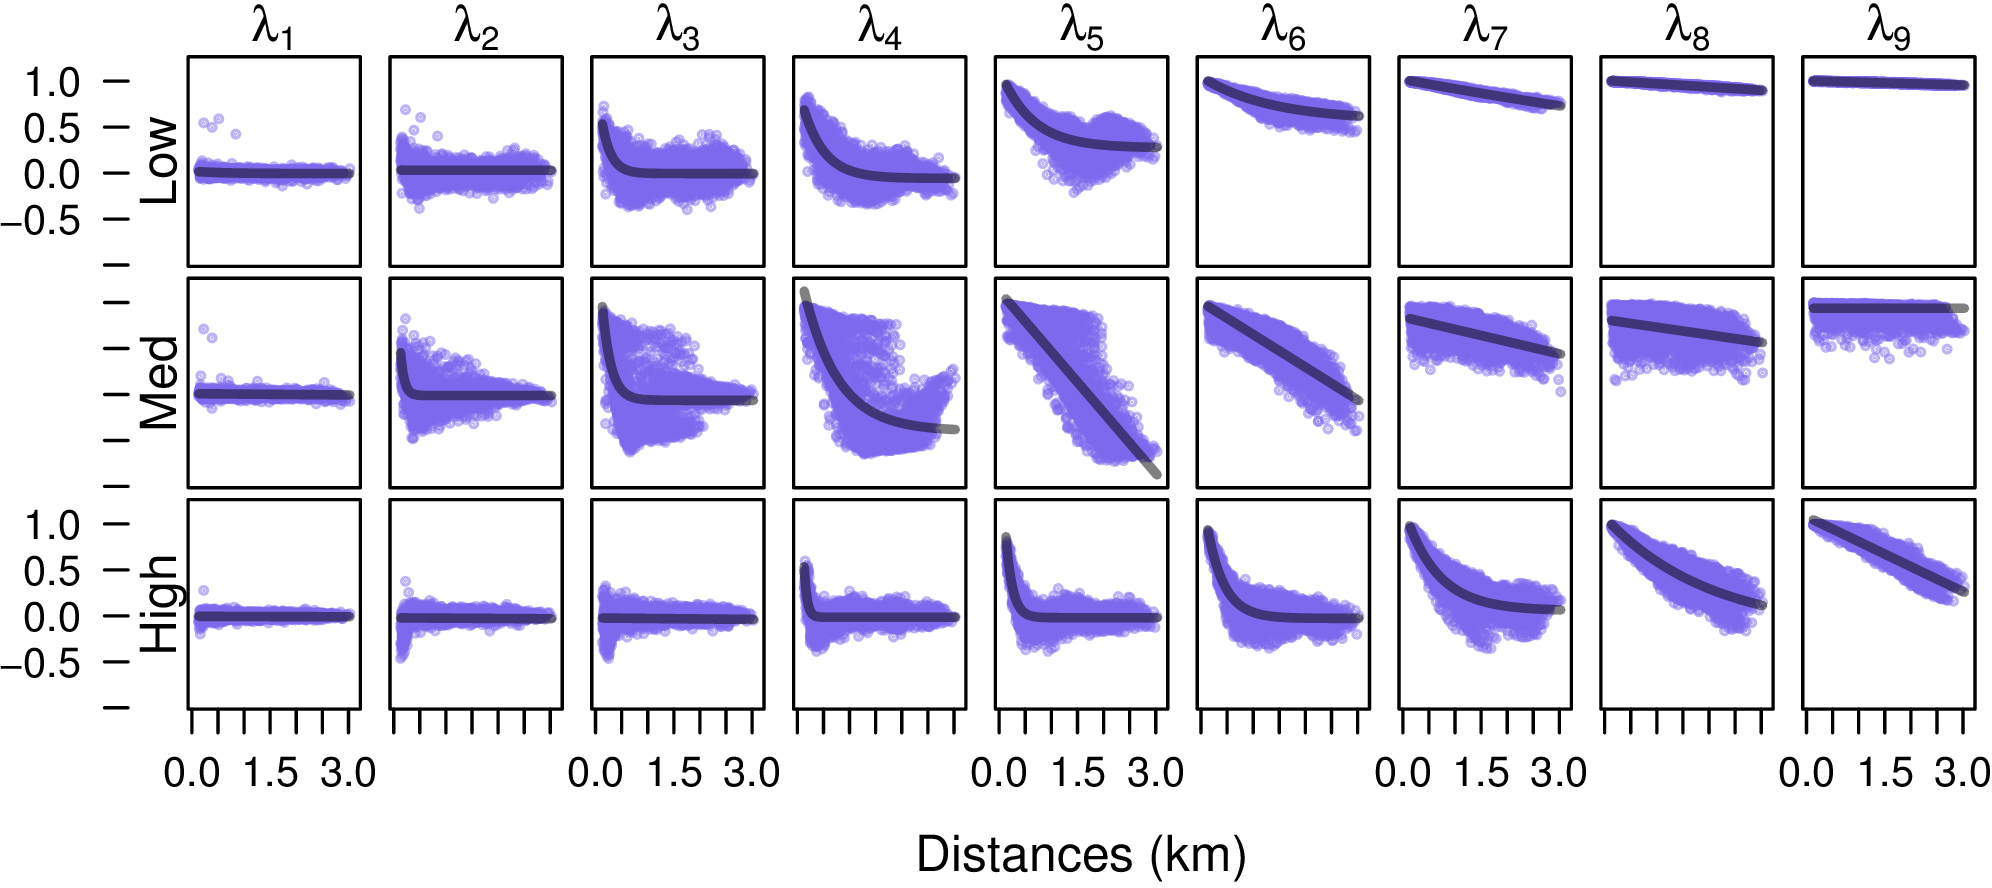
\includegraphics[height=0.5\textheight]{../figs/corDistMatrix_nls.png}};
      \draw[red,ultra thick,rounded corners] (6.5,0) rectangle (10, 0.55\textheight);
    \end{tikzpicture}
  \end{center}
\end{frame}

\subsection{Normativas de red}
\label{sec:org318eeb3}
\begin{frame}[label={sec:orgde5ac3e}]{Normativas de red}
\begin{itemize}
\item La \alert{variabilidad} en escalas de tiempo bajas \alert{puede influir} en mayor o
menor medida en el \alert{funcionamiento de la red eléctrica}.
\item Existencia de \alert{normativas y recomendaciones} para la integración de
sistemas fotovoltaicos en la red.
\item \alert{Ejemplo clásico}: Autoridad Eléctrica de Puerto Rico incluye en su
normativa el concepto de rampa para cuantificar las fluctuaciones
admisibles:
\end{itemize}

\begin{quote}
A 10\% per minute rate (based on AC contracted capacity) limitation shall be enforced. This ramp rate limit applies both to the increase and decrease of power output and is independent of meteorological conditions.
\end{quote}
\end{frame}

\begin{frame}[label={sec:org223a1a1}]{Definiciones de rampas}
Uno de los problemas principales en este requerimiento (y otros similares) es que, aunque \alert{es fácil identificar visualmente una rampa} en una serie temporal de potencia, \alert{no existe consenso en una definición formal} que permita identificarla y cuantificarla.
\end{frame}

\begin{frame}[label={sec:org4ce92b5}]{Ejemplos de definiciones de rampas}
\begin{itemize}
\item Existe una rampa al inicio de un intervalo temporal si la magnitud del cambio en un instante temporal posterior es mayor que un umbral predeterminado.
\end{itemize}
\[ 
\left| P(t +\Delta_t) - P(t)\right| > \psi
\]

\begin{itemize}
\item Existe una rampa en un intervalo temporal si la diferencia entre los
valores máximo y mínimo supera un determinado umbral.
\end{itemize}
\[
\max(\{P_t: t = t_0, \dots, t_0+\Delta_t\}) - \min(\{P_t: t=t_0,
\dots, t_0+\Delta_t\}) > \psi
\]

\begin{itemize}
\item Existe una rampa dentro de un intervalo si el ratio entre el valor absoluto de la diferencia entre las medidas de potencia en dos instantes temporales, y la longitud del intervalo supera un determinado umbral.
\end{itemize}
\[
\frac{\left|P(t + \Delta_t) - P(t)\right|}{\Delta_t} > \psi
\]

\begin{itemize}
\item Existe una rampa en un intervalo si el valor absoluto de la señal de diferencias filtrada (por ejemplo, mediante una media móvil) supera un determinado umbral.
\end{itemize}
\end{frame}

\section{Sistemas de Acumulación}
\label{sec:org3d89284}

\subsection{Fundamentos}
\label{sec:orga6a3e28}
\begin{frame}[label={sec:orge872e02}]{Limitación de rampas}
La limitación de las rampas de los sistemas fotovoltaicos es un
requerimiento que se debe afrontar, principalmente en el caso de las
centrales fotovoltaicas de gran tamaño.

Existen \alert{tres estrategias} principales:
\begin{itemize}
\item el uso de \alert{sistemas de acumulación} energética;
\item \alert{acumulación} energética combinada \alert{con predicción} de rampas;
\item \alert{predicción} de rampas \alert{sin acumulación}.
\end{itemize}
\end{frame}

\begin{frame}[label={sec:orgfc4297e}]{Acumulación o predicción}
La inclusión de sistemas de acumulación conlleva \alert{aumentos en los
costes} de instalación y en la \alert{complejidad y mantenimiento} del
sistema.

Las herramientas de \alert{predicción} de rampas combinadas con \alert{mecanismos de
control en el inversor} fotovoltaico permiten \alert{reducir} el tamaño de la
acumulación necesaria.
\end{frame}

\begin{frame}[label={sec:orgcfcb58a}]{SFCR con acumulación}
\begin{center}
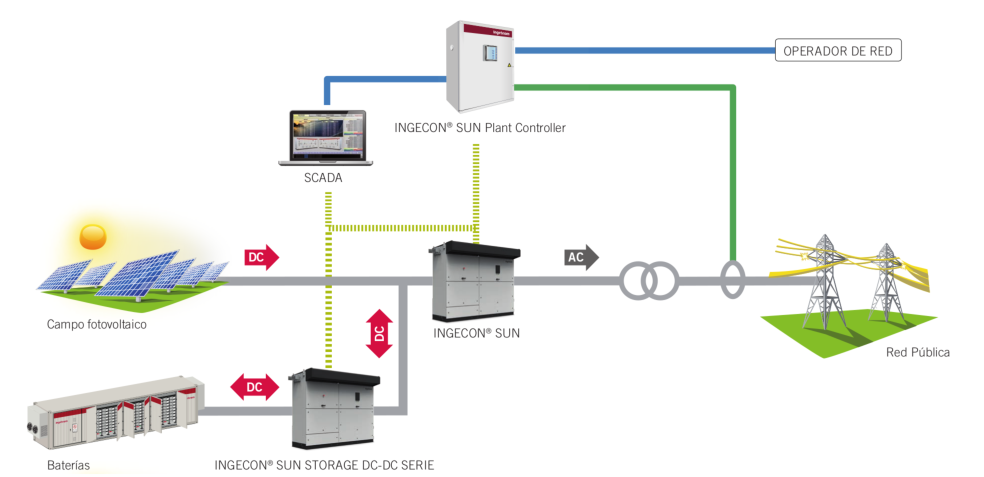
\includegraphics[width=\textwidth]{../figs/EsquemaSFCRAcumulacion.pdf}
\end{center}
\end{frame}

\begin{frame}[label={sec:orgdadf7a4}]{Suavizado de rampas con acumulación}
\begin{center}
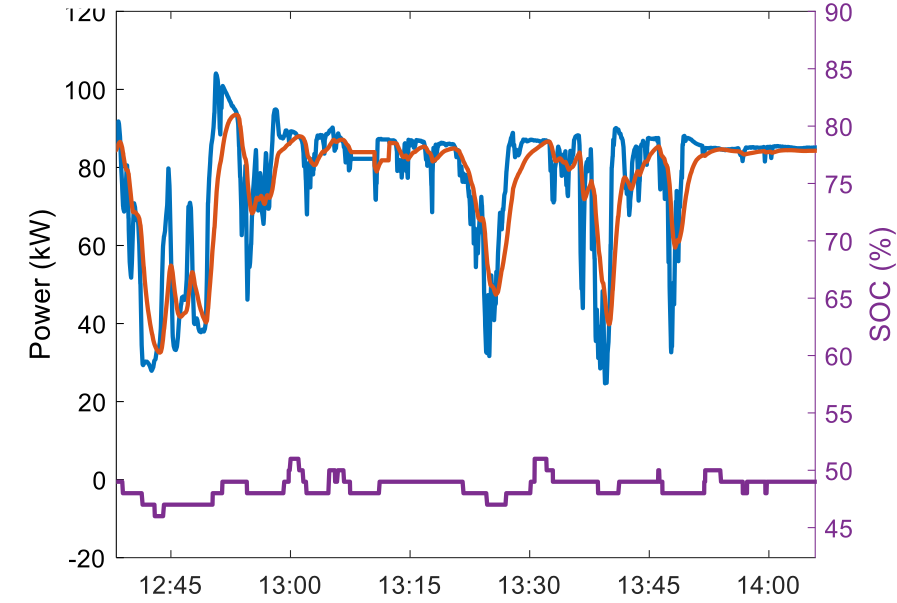
\includegraphics[height=0.9\textheight]{../figs/SuavizadoRampasAcumulacion.png}
\end{center}
\end{frame}

\subsection{Cálculo del sistema de acumulación}
\label{sec:orgcc981ad}

\begin{frame}[label={sec:org4c690a6}]{Objetivos}
\begin{block}{Objetivos}
\begin{itemize}
\item Dimensionar, en \alert{potencia y energía}, la batería mínima necesaria.
\item \alert{Desarrollar estrategias de gestión} que permitan, cumpliendo con la rampa máxima, minimizar el coste de la energía:
\begin{itemize}
\item Minimizar Batería
\item Minimizar Degradación
\item Minimizar Pérdidas
\end{itemize}
\end{itemize}
\end{block}
\end{frame}

\begin{frame}[label={sec:org98ccee7}]{Modelo de la peor fluctuación\footnote{\url{https://dx.doi.org/10.1016/j.solener.2013.10.037}}}
Un pulso de irradiancia se transforma en una exponencial decreciente (la central actúa como filtro paso bajo.

\begin{center}
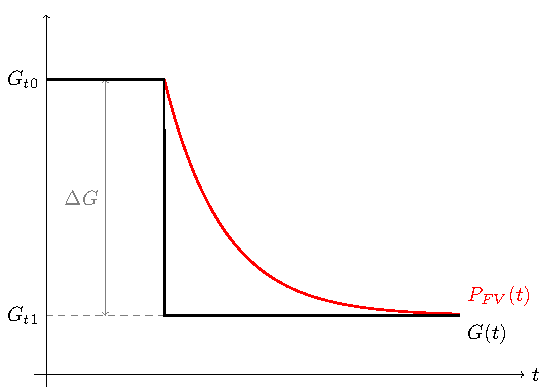
\includegraphics[height=0.7\textheight]{../figs/ModeloPeorFluctuacion0.pdf}
\end{center}
\end{frame}

\begin{frame}[label={sec:org1fb0e28}]{Modelo de la peor fluctuación (2)}
El sistema de acumulación regula la potencia de salida para limitar la rampa. 
\[
  P_{bat} = P_{lim} - P_{FV}
\]

\begin{center}
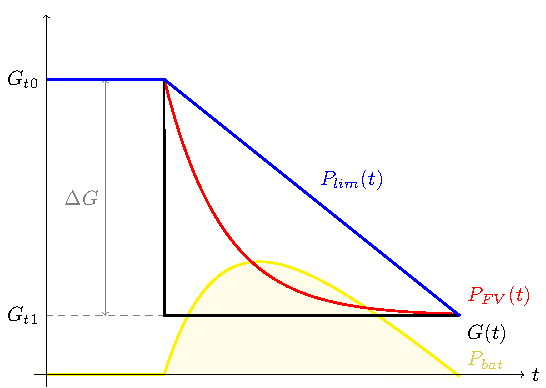
\includegraphics[height=0.75\textheight]{../figs/ModeloPeorFluctuacion.pdf}
\end{center}
\end{frame}

\begin{frame}[label={sec:org5155cd0}]{Modelo de la peor fluctuación (3)}
\begin{columns}
\begin{column}{0.4\columnwidth}
\begin{center}
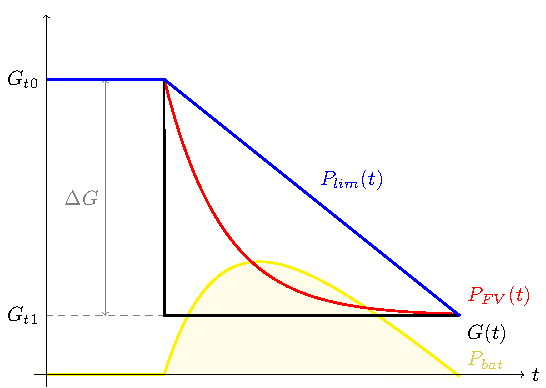
\includegraphics[width=\textwidth]{../figs/ModeloPeorFluctuacion.pdf}
\end{center}
\end{column}

\begin{column}{0.6\columnwidth}
\[
  P_{FV}(t) = 90 \cdot \exp(-t/\tau) + 10
\]

\[
  \tau = a \cdot L_{min} - b
\]

\begin{itemize}
\item \(\tau [\unit{\second}]\): constante de tiempo de la fluctuación
\item \(L_{min} [\unit{\kilo\meter}]\): dimensión menor de la central
\end{itemize}
\end{column}
\end{columns}
\end{frame}

\begin{frame}[label={sec:org4cff633}]{Modelo de la peor fluctuación (y 4)}
\begin{columns}
\begin{column}{0.4\columnwidth}
\begin{center}
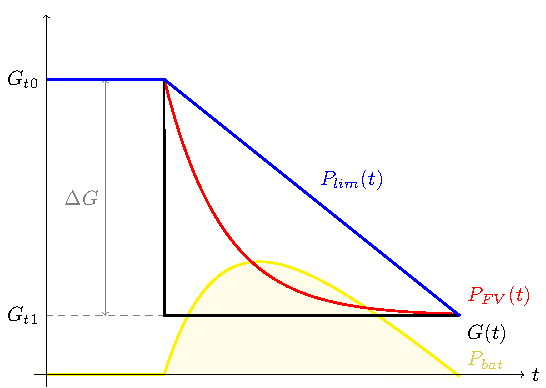
\includegraphics[width=\textwidth]{../figs/ModeloPeorFluctuacion.pdf}
\end{center}
\end{column}

\begin{column}{0.6\columnwidth}
\[
  P_{bat,max} = \frac{P_g^*}{100} \cdot \left(90 - \tau \cdot RR_{max} \cdot \left( 1 + \ln\frac{90}{\tau \cdot RR_{max}}\right) \right)
\]

\[
  E_{bat} = \frac{0.9 \cdot P_g^*}{3600} \cdot \left( \frac{90}{2 \cdot RR_{max}} - \tau \right)
\]

\begin{itemize}
\item \(P_g^* [\unit{\kilo\watt}]\): potencia del generador fotovoltaico
\item \(RR_{max} [\unit{\%\per\sec}]\): límite de rampa en potencia
\item \(P_{bat,max} [\unit{\kilo\watt}]\): potencia máxima del sistema de acumulación
\item \(E_{bat} [\unit{\kilo\watthour}]\): capacidad del sistema de acumulación.
\end{itemize}
\end{column}
\end{columns}
\end{frame}

\begin{frame}[label={sec:org402d027}]{Ejemplo: cálculo de potencia}
Datos:
\begin{align*}
  P_g^* &= \qty{38.5}{\mega\watt}\\
  L_{min} &= \qty{1.786}{\kilo\meter}\\
  a &= 42\\
  b &= 0.55\\
  RR_{max} &= \qty{10}{\%\per\min}
\end{align*}
Resultados:
\begin{align*}
  \tau &= 42 \cdot \num{1.786} - \num{0.55} = \qty{74.46}{\second}\\
  P_{bat,max} &= \frac{\num{38500}}{100} \cdot \left(90 - \num{74.46} \cdot (10/60) \cdot \left( 1 + \ln\frac{90}{\num{74.46} \cdot (10/60)}\right) \right) = \qty{20.4}{\mega\watt}\\
  \frac{P_{bat,max}}{P_g^*} &= \num{0.53}
\end{align*}
\end{frame}

\begin{frame}[label={sec:org10fabc7}]{Ejemplo: cálculo de capacidad}
Datos:
\begin{align*}
  P_g^* &= \qty{38.5}{\mega\watt}\\
  L_{min} &= \qty{1.786}{\kilo\meter}\\
  RR_{max} &= \qty{10}{\%\per\min}
\end{align*}
Resultados:
\begin{align*}
  E_{bat} &= \frac{\num{0.9} \cdot \num{38500}}{\num{3600}} \cdot \left( \frac{90}{2 \cdot (10/60)} - \num{74.46} \right) = \qty{1882.05}{\kilo\watthour}\\
  \frac{E_{bat}}{P_g^*} &= \qty{0.049}{\hour} 
\end{align*}
\end{frame}

\subsection{Tecnologías de acumulación}
\label{sec:org1cad59e}

\begin{frame}[label={sec:org3697876}]{Tecnologías de acumulación\footnote{\href{https://ease-storage.eu/publication/ease-eera-energy-storage-technology-development-roadmap-2017/}{EASE-EERA Energy Storage Technology Development Roadmap}}}
\begin{center}
  \begin{tikzpicture}
    \node[anchor=south west,inner sep=0] at (0,0) {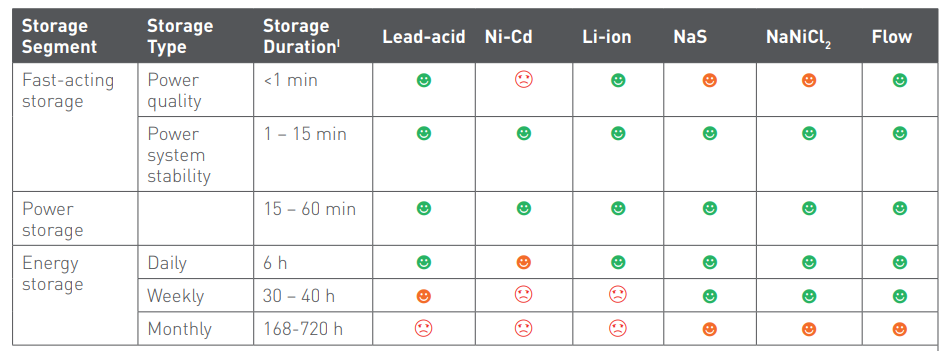
\includegraphics[height=0.5\textheight]{../figs/ComparativaTecnologiasAcumulacion.png}};
      \draw[red,ultra thick,rounded corners] (7,0) rectangle (8.2, 0.5\textheight);
    \end{tikzpicture}
  \end{center}
\end{frame}

\begin{frame}[label={sec:orgaed06e3}]{Tecnologías de acumulación\footnote{\url{https://dx.doi.org/10.1016/j.apenergy.2014.09.081}}}
\begin{center}
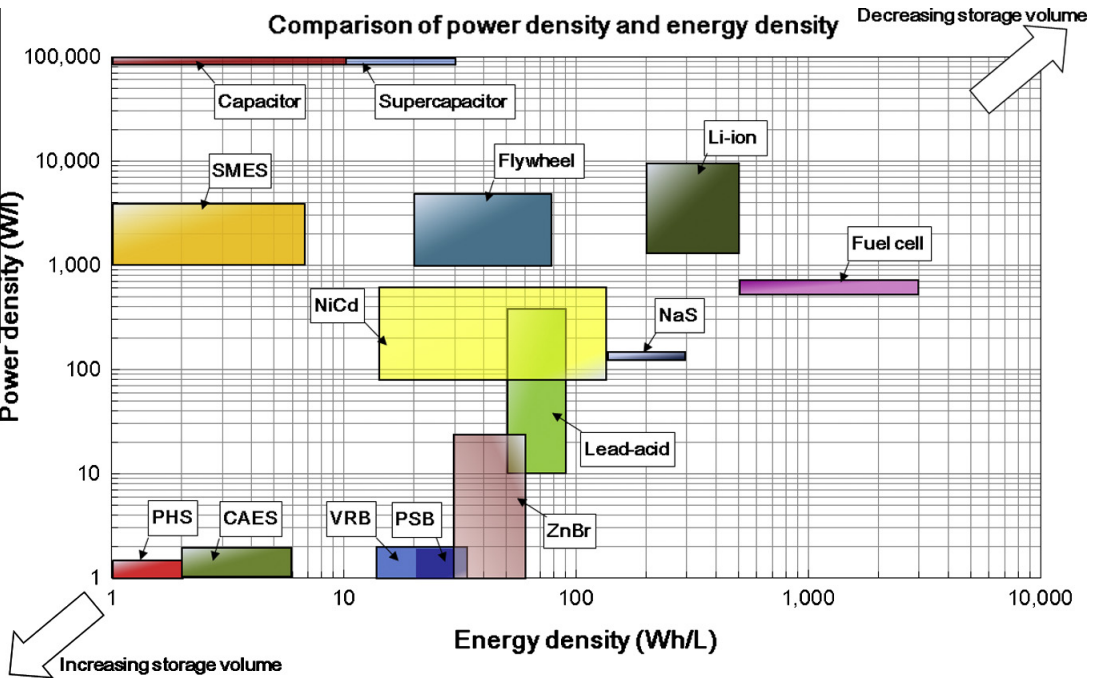
\includegraphics[height=0.8\textheight]{../figs/SistemasAcumulacion_DensidadPotenciaEnergia.png}
\end{center}
\end{frame}

\begin{frame}[label={sec:orgce9eb2c}]{Otros usos del sistema de acumulación}
Los sistemas de acumulación pueden proporcionar servicios adicionales\footnote{\url{https://dx.doi.org/10.1016/j.apenergy.2020.115213}}:

\begin{itemize}
\item \alert{Regulación de frecuencia}: mantener la frecuencia de la red dentro de unos límites.
\item \alert{Emulación de inercia}: evitar cambios rápidos tras una descompensación de potencia.
\item \alert{\emph{Black start}}: recuperar el sistema eléctrico después de un apagón.
\item \alert{\emph{Capacity Firming}}: mantener el nivel de generación durante un período de tiempo.
\item \alert{\emph{Arbitrage}} o \emph{time-shift}: comprar energía cuando es barata, vender cuando es cara.
\end{itemize}
\end{frame}
\end{document}
